\chapter{\ifproject%
\ifenglish Project Structure and Methodology\else โครงสร้างและขั้นตอนการทำงาน\fi
\else%
\ifenglish Project Structure\else โครงสร้างของโครงงาน\fi
\fi
}

ในบทนี้จะกล่าวถึงหลักการ และการออกแบบระบบ

\makeatletter

% \renewcommand\section{\@startsection {section}{1}{\z@}%
%                                    {13.5ex \@plus -1ex \@minus -.2ex}%
%                                    {2.3ex \@plus.2ex}%
%                                    {\normalfont\large\bfseries}}

\makeatother
%\vspace{2ex}
% \titleformat{\section}{\normalfont\bfseries}{\thesection}{1em}{}
% \titlespacing*{\section}{0pt}{10ex}{0pt}

\section{เนื้อหา}

\subsection{เนื้อเรื่อง}

เกมนี้มีเนื่อเรื่องและสถานที่อยู่ในยุโรปยุคกลาง ตามความเชื่อที่ว่า ปีศาจสามารถปลอมแปลงเป็นสัตว์ชนิด
หนึ่ง อาศัยอยู่ในป่ารกร้าง หน้าที่ของผู้เล่นคือ ต้องไปปราบปีศาจร้ายและทําให้ผู้คนปลอดภัย

\subsection{ดนตรีและเสียงประกอบ}

เกมนี้มีเสียงประกอบที่สร้างความสมจริงและความสยองขวัญ โดยมีเสียงประกอบทั้งหมด 2 ชนิด ได้แก่ ดนตรี ซาวด์เอฟเฟค
\begin{itemize}
  \item เสียงดนตรี: จะถูกเล่นเมื่อผู้เล่นเห็นฝั่งตรงข้ามหรือโจมตีกัน โดยจะเป็นเสียงดนตรีที่สร้างความระทึก และจะหยุดเล่นเมื่อผู้เล่นหลบหนีไปห่างจากฝั่งตรงข้าม
  \item เสียงซาวด์เอฟเฟค: จะถูกเล่นเมื่อผู้เล่นทำการกระทำต่าง ๆ
\end{itemize}

เสียงซาวด์เอฟเฟคจะเป็นเสียงแบบ 3 มิติ ที่มีระยะการได้ยินที่เหมาะสม ซึ่งจะทำให้ผู้เล่นสามารถระบุตำแหน่งของฝ่ายตรงข้ามได้ 
นอกจากนี้แล้วเสียงซาวน์เอฟเฟคการเดินและวิ่งจะขึ้นอยู่กับพื้นผิวที่ผู้เล่นกำลังเคลื่อนที่อยู่

\subsection{ฉาก}

สถานที่ของเกมคือป่าสนแห้งแล้งแห่งหนึ่งในยุโรป ขนาดของแผนที่ คือ 400 x 400 เมตร ประกอบไปด้วยทะเลสาบ 
น้ำตก ลำธาร ป่าสน และเนินเขา รวมถึงมีบ้านเก่า ๆ ที่ถูกทิ้งไว้ ซึ่งสามารถเป็นจุดนัดพบได้ เวลาของเกมคือช่วงกลางคืน 
สถานที่นอกจากมืดแล้วยังมีหมอกที่หนาแน่น ทำให้มองเห็นได้ไม่ชัดเจน เพื่อเพิ่มความสยองขวัญให้กับผู้เล่น

\begin{figure}[p]
  \begin{center}
  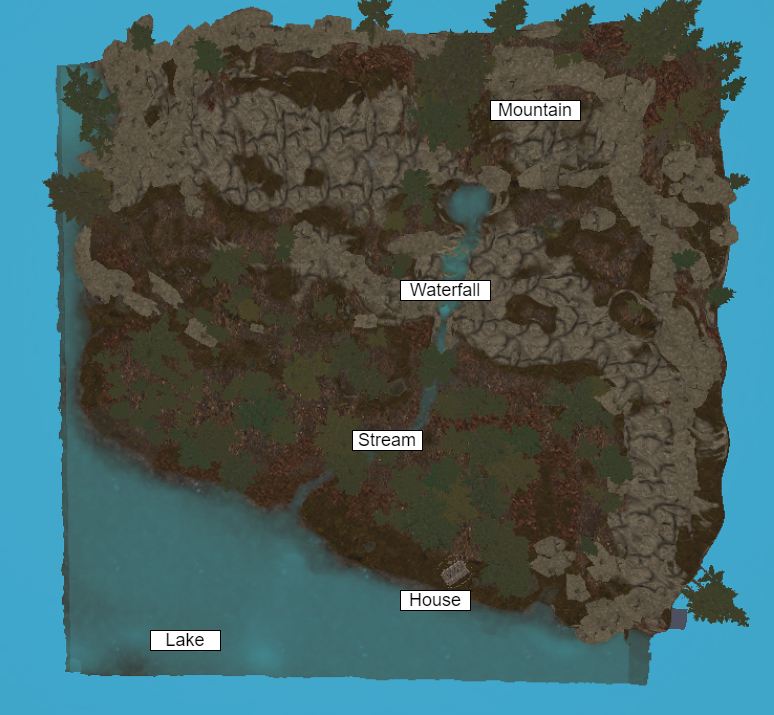
\includegraphics[width=0.7\textwidth]{./img/scene/WitchHunter-Map.png}
  \end{center}
  \caption[ภาพมุมสูงแสดงตำแหน่งของสถานที่ต่าง ๆ
  และภูมิประเทศของฉากในเกม]{ภาพมุมสูงแสดงตำแหน่งของสถานที่ต่าง ๆ
  และภูมิประเทศของฉากในเกม}
  \label{ภาพมุมสูงแสดงตำแหน่งของสถานที่ต่าง ๆ
  และภูมิประเทศของฉากในเกม}
\end{figure}

\begin{figure}[p]
  \begin{center}
  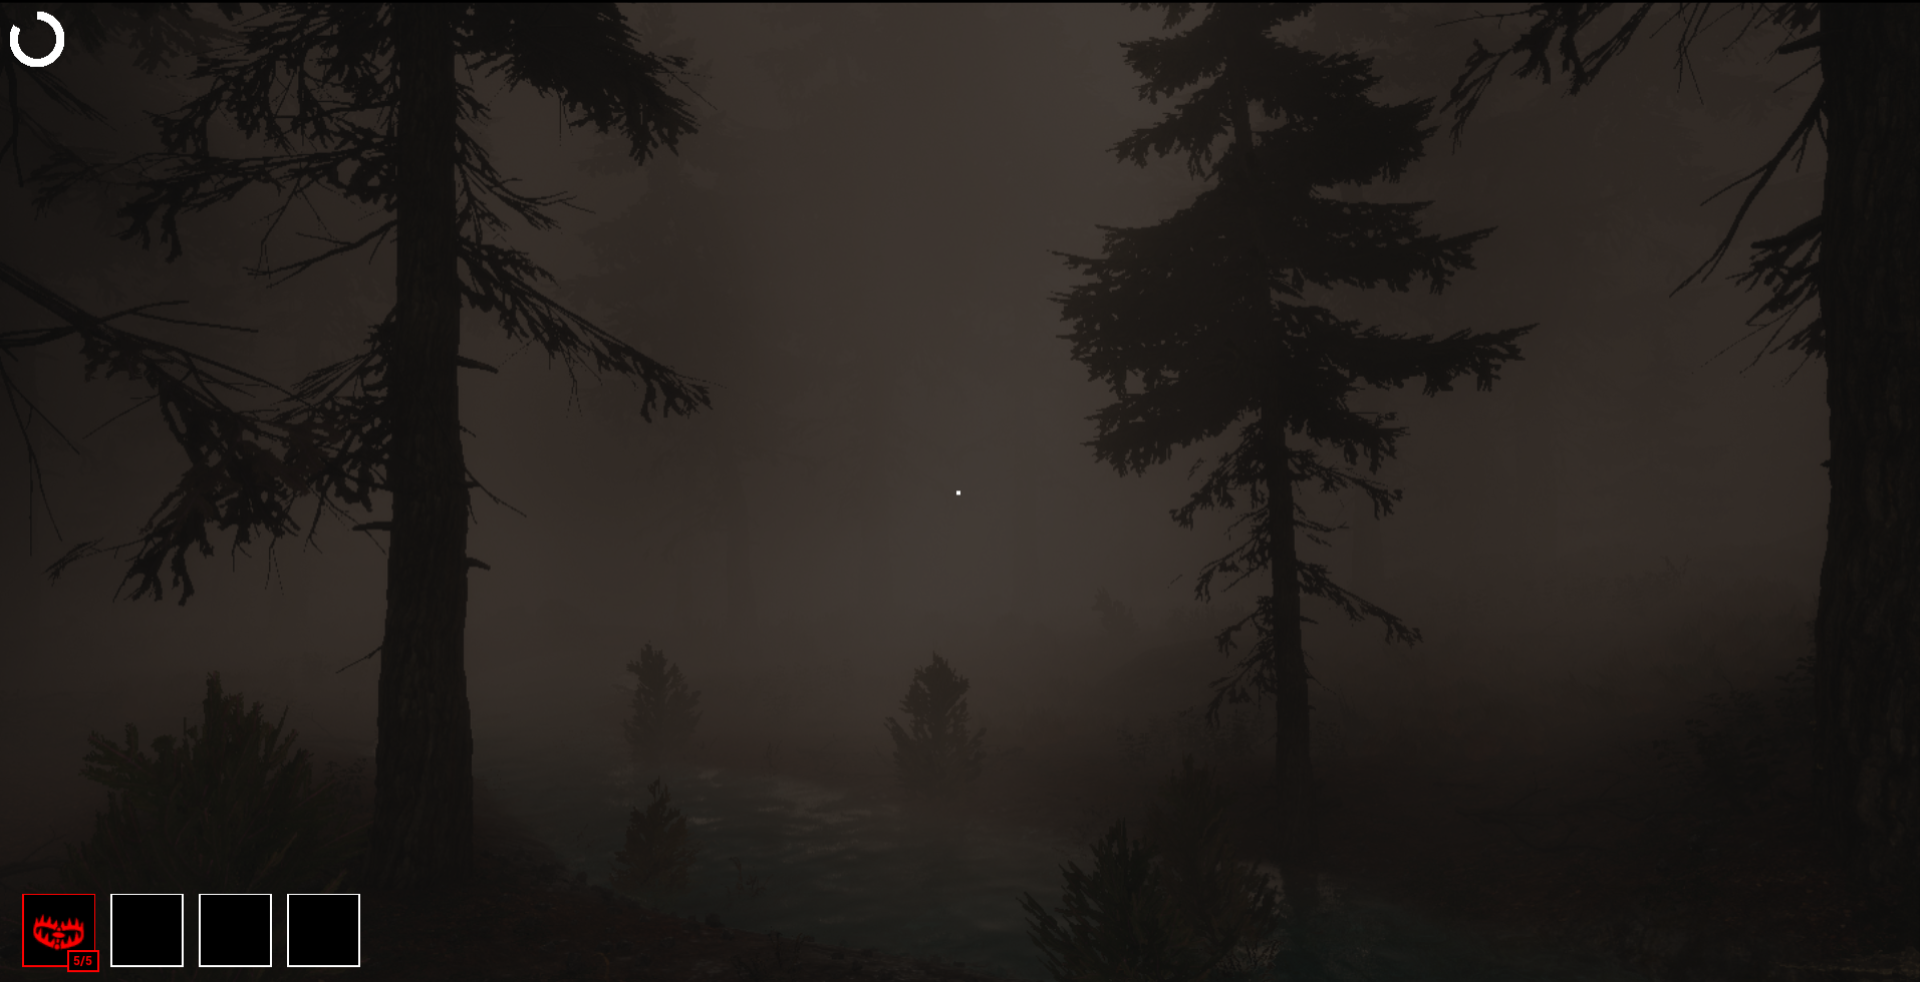
\includegraphics[width=\textwidth]{./img/scene/atmosphere.png}
  \end{center}
  \caption[ภาพบรรยากาศภายในเกม]{ภาพบรรยากาศภายในเกม}
  \label{ภาพบรรยากาศภายในเกม}
\end{figure}

\subsection{ตัวละคร}

ในเกมนี้มีตัวละครทั้งหมด 3 ตัว ได้แก่ 2 ตัวของฝ่าย Hunters และ 1 ตัวของฝ่าย Witch ตัวละครถูกสร้างขึ้นโดยดัดแปลงจาก
โมเดลเสื้อผ้าและร่างกายที่มีอยู่แล้วในโปรแกรม Reallusion Character Creator

\subsubsection{ตัวละครฝ่าย Hunters}

แบ่งเป็น 2 ตัวละคร ชายและหญิง ซึ่งเป็นนายพรานและมีความสามารถเหมือนกันทั้งคู่

\begin{figure}
  \centering
  \begin{subcaptionblock}{.4\textwidth}
    \centering
    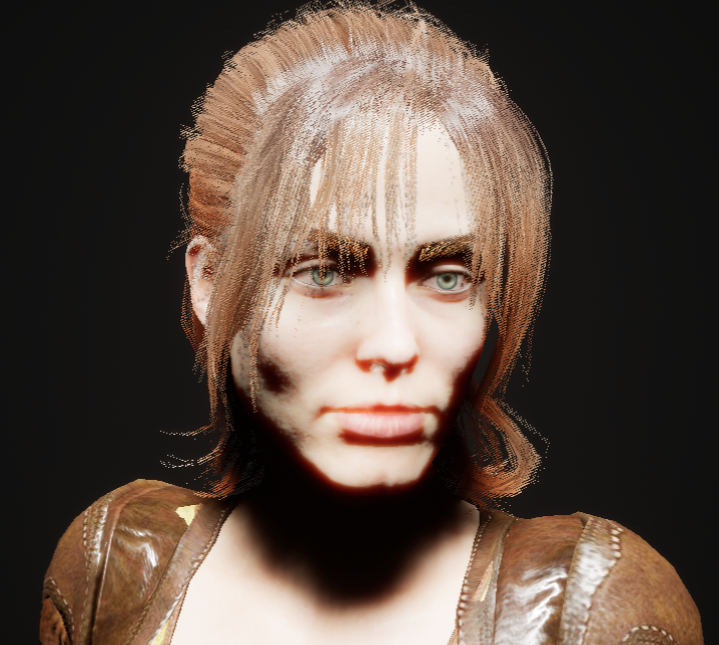
\includegraphics[width=.8\linewidth]{./img/characters/emma_face.png}
    \caption{ภาพใบหน้าตัวละคร Hunter หญิง}\label{ภาพใบหน้าตัวละคร Hunter หญิง}
  \end{subcaptionblock}%
  \begin{subcaptionblock}{.4\textwidth}
    \centering
    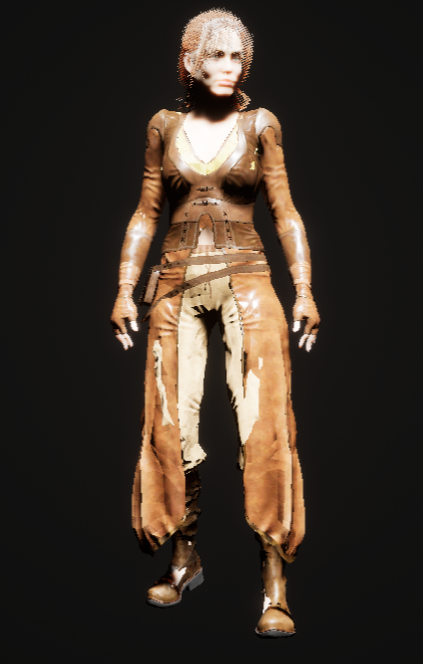
\includegraphics[width=.8\linewidth]{./img/characters/emma_full.png}
    \caption{ภาพเต็มตัวตัวละคร Hunter หญิง}\label{ภาพตัวเต็มตัวละคร Hunter หญิง}
  \end{subcaptionblock}%
  \caption{ภาพตัวละคร Hunter หญิง}\label{ภาพตัวละคร Hunter หญิง}
\end{figure}

\begin{figure}
  \centering
  \begin{subcaptionblock}{.4\textwidth}
    \centering
    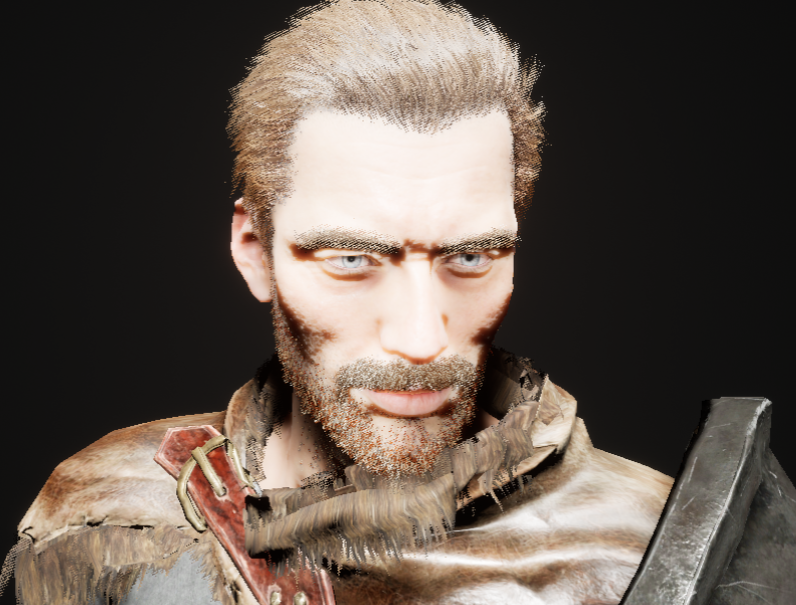
\includegraphics[width=.8\linewidth]{./img/characters/eric_face.png}
    \caption{ภาพใบหน้าตัวละคร Hunter ชาย}\label{ภาพใบหน้าตัวละคร Hunter ชาย}
  \end{subcaptionblock}%
  \begin{subcaptionblock}{.4\textwidth}
    \centering
    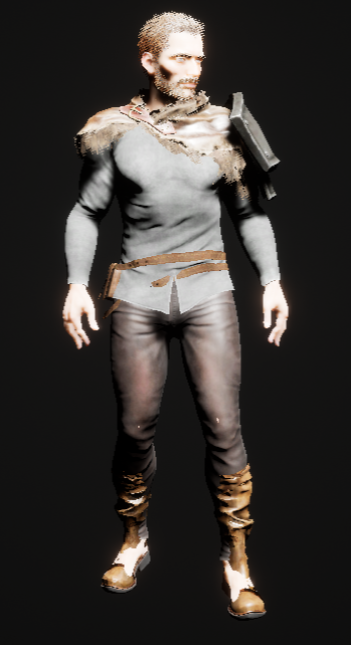
\includegraphics[width=.8\linewidth]{./img/characters/eric_full.png}
    \caption{ภาพเต็มตัวตัวละคร Hunter ชาย}\label{ภาพตัวเต็มตัวละคร Hunter ชาย}
  \end{subcaptionblock}%
  \caption{ภาพตัวละคร Hunter ชาย}\label{ภาพตัวละคร Hunter ชาย}
\end{figure}

\subsubsection{ตัวละครฝ่าย Witch}

ร่างของแม่มดจะเป็นหญิงแก่หน้าตาอัปลักษณ์ที่มีศีรษะหันไปด้านหลังและเดินถอยหลัง

\begin{figure}
  \centering
  \begin{subcaptionblock}{.4\textwidth}
    \centering
    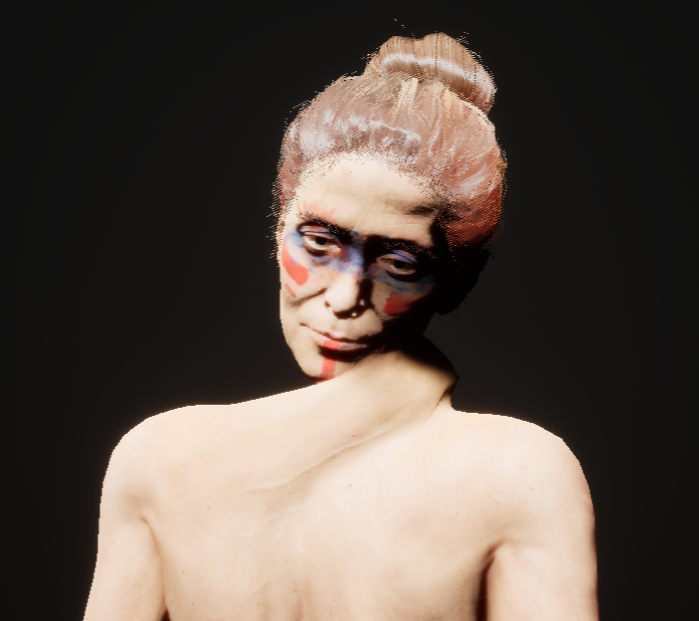
\includegraphics[width=.8\linewidth]{./img/characters/witch_face.png}
    \caption{ภาพใบหน้าตัวละคร Witch}\label{ภาพใบหน้าตัวละคร Witch}
  \end{subcaptionblock}%
  \begin{subcaptionblock}{.4\textwidth}
    \centering
    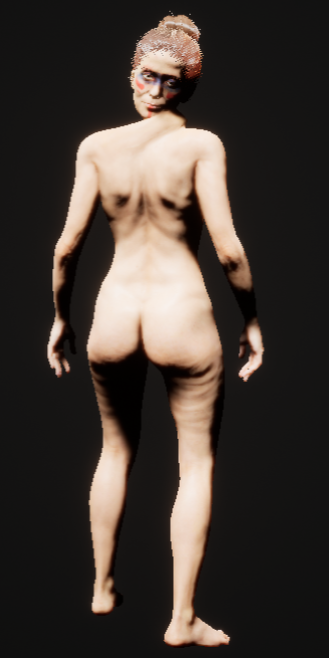
\includegraphics[width=.8\linewidth]{./img/characters/witch_full.png}
    \caption{ภาพเต็มตัวตัวละคร Witch}\label{ภาพตัวเต็มตัวละคร Witch}
  \end{subcaptionblock}%
  \caption{ภาพตัวละคร Witch}\label{ภาพตัวละคร Witch}
\end{figure}

\begin{figure}[p]
  \begin{center}
  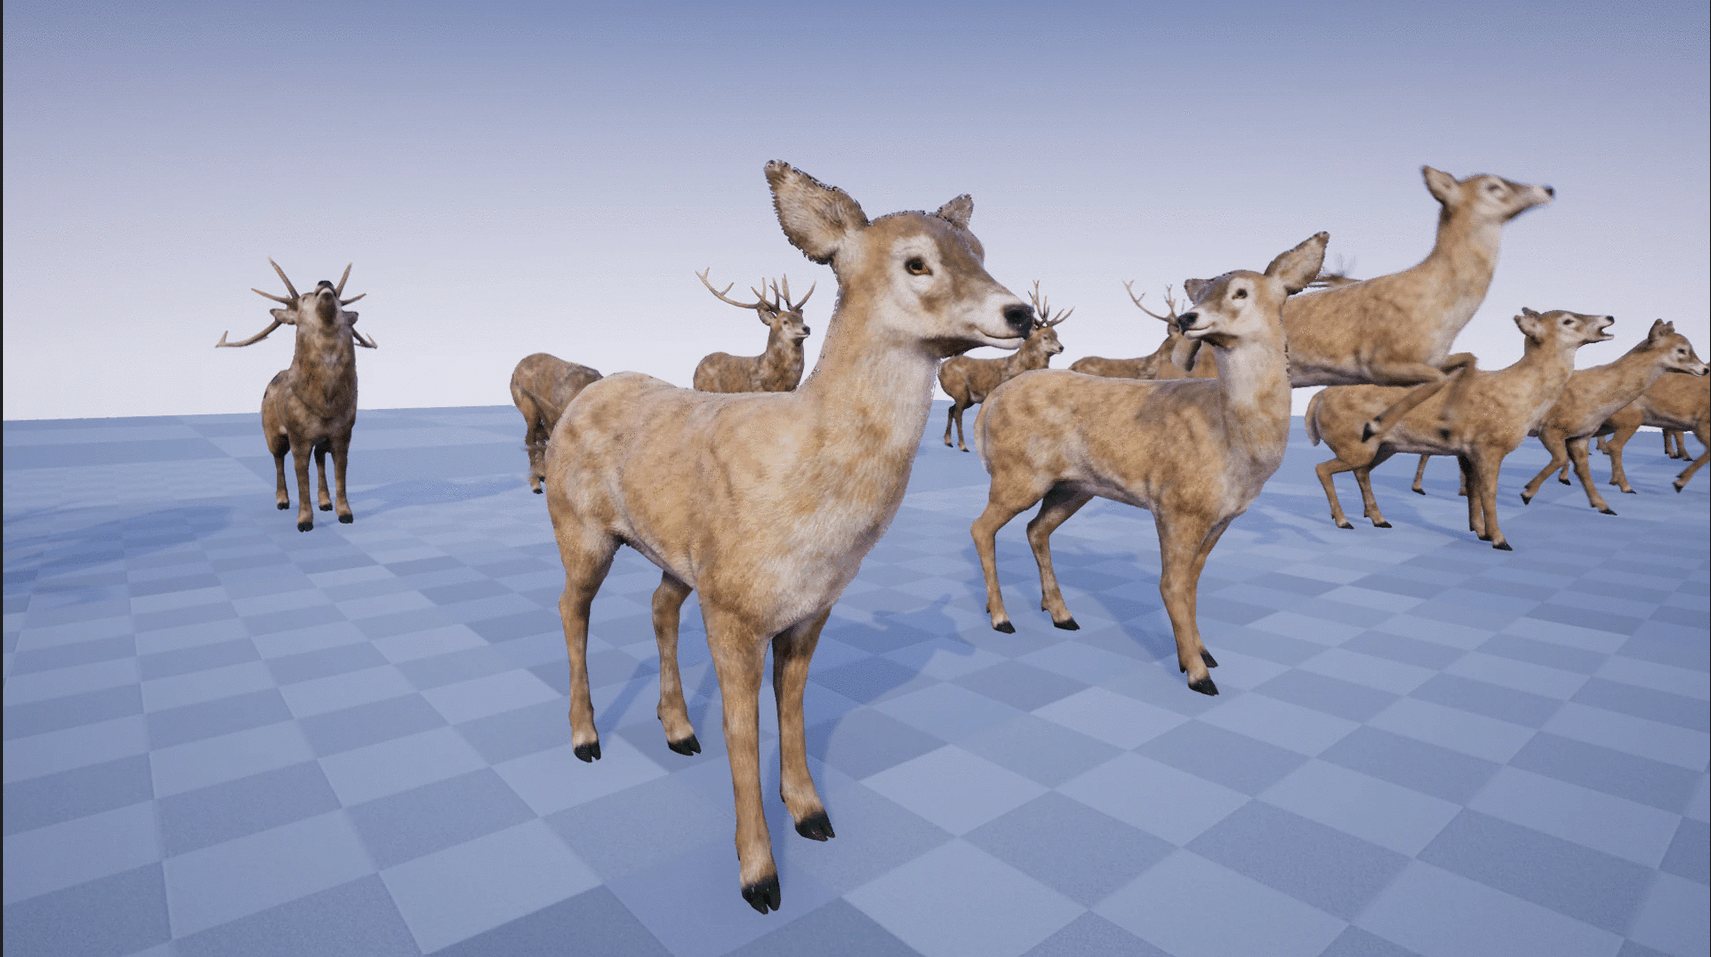
\includegraphics[width=\textwidth]{./img/characters/deerdoe.png}
  \end{center}
  \caption[ภาพตัวละครกวาง]{ภาพตัวละครกวาง}
  \label{ภาพตัวละครกวาง}
\end{figure}

\subsubsection{ตัวละครกวาง}

กวางสามารถนอน กิน และเดินไปมาได้ อีกทั้งยังสามารถวิ่งหนี Hunter ที่พยายามจับได้อีกด้วย นอกเหนือจากนี้แล้วกวางยังสามารถถูกควบคุมได้โดย Witch

\section{วิธีการเล่น}

เพชฌฆาตแม่มด (Witch Hunter) เป็นเกมสยองขวัญแบบหลายผู้เล่น 2vs1 โดยผู้เล่นแบ่งออกเป็น 2 ฝั่ง 
ฝั่งของ Hunters ประกอบด้วยผู้เล่น 2 คน ต้องร่วมมือกันทำภารกิจที่กำหนดไว้ ซึ่งก็คือการจับกวางที่เป็นลูกสมุน
ของแม่มด แล้วนำเลือดมาทำพิธี 6 ครั้งตามจุดที่กำหนดไว้แบบสุ่ม ในขณะที่ฝั่ง Witch ซึ่งประกอบด้วยผู้เล่น 1 คน
ต้องขัดขวางฝ่าย Hunters ไม่ให้ทำภารกิจสำเร็จ โดยการปลอมตัวเป็นกวางเพื่อหลอกล่อ Hunters และทำการ
โจมตีด้วยเวทมนต์

\subsection{การเล่นของฝ่าย Hunters}

\subsubsection{การจับกวาง}

สามารถจับกวางด้วยการปามีดศักดิ์สิทธิ์หรือวางกับดักทิ้งไว้ เมื่อกวางถูกโจมตีหรือถูกกับดักจะล้มลง Hunter มีหน้าที่
ที่ต้องทำการสกัดเลือดจากตัวกวางที่ล้มลงไป กวางแต่ละตัวไม่ได้นิ่งเฉย แต่สามารถนอน กิน หรือเดินไปมาได้ ซึ่ง
Hunter ต้องอาศัยความละมุมละม่อมในการจับกวางเพราะถ้าหากวิ่งเข้าไปหาหรือเดินเข้าไปใกล้เกินไป กวางจะตกใจ
วิ่งหนี ซึ่งอีกฝั่งอาจสังเกตุเห็นความผิดปกตินี้และสามารถระบุตำแหน่งของ Hunter ได้

\subsubsection{การทำพิธี}

เมื่อ Hunter ได้ทำการสกัดเลือดจากกวางแล้ว Hunter สามารถเลือกทำพิธีกรรม โดยการนำเลือดที่สกัดไปทำพิธี
ที่จุดที่กำหนดไว้จุดไหนก็ได้ ซึ่งจะมีจุดที่กำหนดไว้ 3 จุด และจะมีการสุ่มจุดที่จะทำพิธีในแต่ละเกม ซึ่งเมื่อผู้เล่นคนนั้น
ทำพิธีเสร็จสิ้น 1 ครั้ง เขาจะได้รับการฟื้นฟู HP 1 ระดับ ในการทำพิธี 1 ครั้ง จะใช้เวลา 30 วินาที สามารถยกเลิก
การทำพิธีได้ แต่ต้องเริ่มทำพิธีใหม่ทั้งหมดใหม่

\subsubsection{การโจมตี Witch}

Hunter สามารถโจมตี Witch ได้โดยการปามีดศักดิ์สิทธิ์ใส่ Witch การโจมตี Witch นี้จะทำให้ Witch สะดุด
และเดินช้าลง รวมถึงทำให้มองไม่เห็นแต่เพียงแค่ช่วงเวลาสั้น ๆ เท่านั้น ในระหว่างนี้ Hunter สามารถวิ่งไปแอบหลัง
ต้นไม้ ก้อนหิน เพื่อหลุดจากการไล่ล่าและทำพิธีต่อ

\subsubsection{ระบบ Inventory}

Hunter สามารถเก็บ ใช้ และดร็อปไอเทมได้ ทำให้สามารถส่งต่อไอเทมให้ผู้เล่นอีกคนได้อีกด้วย โดยไอเทมที่
สามารถเก็บและใช้ได้ มีดังนี้
\begin{enumerate}
  \item มีดศักดิ์สิทธิ์ มีให้ 10 เล่ม ปาแล้วสามารถเก็บมาใช้ซ้ำได้
  \item กับดักสัตว์ มีให้ 5 อัน สามารถวางไว้ได้ทุกที่ และสามารถเก็บมาใช้ซ้ำได้
  \item หลอดบรรจุเลือดของกวางที่ได้หลังจากการสกัดเลือด
\end{enumerate}

\subsubsection{ระบบ HP}

HP ของ Hunter มี 3 ระดับ โดยเมื่อถูกโจมตีจาก Witch จะลดลง 1 ระดับ และสามารถฟื้นฟู HP ได้
ด้วยการทำพิธี 1 ครั้ง ซึ่งจะได้รับการฟื้นฟู HP 1 ระดับต่อการทำพิธีหนึ่งครั้ง แต่ไม่สามารถฟื้นฟู HP จนมากกว่า 3 
ระดับได้

ในเกมจะไม่แสดงหลอดเลือดแต่แสดงเป็น Vignette Effect สีแดงบนจอ ซึ่งจะรุนแแรงขึ้นเรื่อย ๆ ตามระดับ HP 
ที่ลดลงไป

\subsubsection{ระบบชุบชีวิต}

เมื่อ Hunter ไม่เหลือ HP แล้ว จะเข้าสู่สถานะชุบชีวิต Hunter จะเกิดใหม่เป็นร่างวิญญาณ ณ ร่างของผู้เล่นอีกคน 
สามารถเลือกที่จะเกิดใหม่ด้วยการเดินกลับไปสิงร่างเดิม หรือเลือกที่จะไม่เกิดใหม่แต่เล่นเป็น Spectator ได้ ผู้เล่น
คนอื่น ๆ จะไม่เห็น Hunter ในร่างวิญญาณนี้ Hunter 1 คนสามารถชุบชีวิตได้เพียง 1 ครั้งเท่านั้น

\subsection{การเล่นของฝ่าย Witch}

\subsubsection{การโจมตี Hunter}

Witch สามารถโจมตี Hunter ได้โดยการใช้เวทมนต์ 2 แบบ แบบระยะใกล้และระยะไกล โดยเมื่อโจมตีแล้ว 
Hunter จะลด HP ลง 1 ระดับ

\begin{enumerate}
  \item การโจมตีระยะใกล้ด้วยไอพิษ (Breath of Death): สามารถโจมตีได้ในระยะ 1-2 เมตร
  \item การโจมตีระยะไกลด้วยลูกไฟ (Inferno Soul): สามารถโจมตีในระยะไกลเท่าไหร่ก็ได้ การโจมตี
  เป็นรูปแบบของการยิงเวทมนต์ไฟ (Fire Ball) โดยจะต้องมีการชาร์จพลังให้เต็มก่อนที่จะโจมตีในทุกครั้ง
\end{enumerate}

\subsubsection{การเคลื่อนย้ายร่างไปเป็นกวาง}

Witch สามารถกดดูตำแหน่งและการเคลื่อนที่ของกวางในแมพได้ (Deer Vision) ซึ่งสามารถใช้เลือกกวางที่จะ
ย้ายร่างไปสิงได้ ความสามารถนี้สามารถใช้ได้ทุก ๆ 60 วินาที ในขณะเป็นกวางอยู่ ผู้เล่นไม่สามารถทำการโจมตีอีก
ฝั่งได้ ต้องกลับมาเป็นร่าง Witch เดิมก่อนทำการโจมตี ถ้าหากกวางที่ผู้เล่นสิงอยู่ถูกโจมตีจะทำให้วิญญาณกลับมา
เป็นร่างเดิมทันที

\subsubsection{ความสามารถพิเศษอื่น ๆ}

\begin{itemize}
  \item สามารถมองเห็นตำแหน่งของจุดทำพิธีตอนเริ่มเกมได้
  \item สามารถได้ยินเสียงจุดทำพิธีและการทำพิธีได้ในระยะที่ค่อนข้างไกล
\end{itemize}


\subsection{เงื่อนไขการจบเกม}

\subsubsection{ฝ่าย Hunters ชนะ}

ฝ่าย Hunters ชนะเมื่อทำพิธีได้ครบ 6 ครั้ง ภายในเวลาที่กำหนดไว้

\subsubsection{ฝ่าย Witch ชนะ} 

ฝ่าย Witch ชนะเมื่อ Hunter ทุกคนไม่สามารถชุบร่างใหม่ได้แล้วหรือ Hunter ทุกคนเสียชีวิตกลายเป็นร่างวิญญาณ
ทั้งหมด หรือฝ่าย Hunters ไม่สามารถทำพิธีได้ครบ 6 ครั้งภายในเวลาที่กำหนดไว้

\section{การออกแบบระบบ}

เกมนี้ถูกพัฒนาโดยใช้ Unreal Engine version 5.1.1 เพื่อให้หน้าภาพและบรรยากาศที่สวยงามและสมจริง
อีกทั้ง Game Engine นี้ยังรองรับการพัฒนาเกมแบบ Multiplayer ได้ดี และยังมีเครื่องมือที่สามารถช่วยในการพัฒนา

\subsection{การออกแบบระบบ Multiplayer}

เกมนี้ถูกออกแบบให้เล่นแบบ Multiplayer โดยมีการเชื่อมต่อผ่าน Local Area Network (LAN) เท่านั้น
โดยจะมี 1 ผู้เล่น เป็น Host ทำหน้าที่เป็นทั้ง Server และ Client เรียกว่า Listen Server
\begin{itemize}
  \item Server มีหน้าที่เป็นตัวกลางในการเชื่อมต่อระหว่างผู้เล่นทั้งหมด ควบคุมการเกิดเหตุการณ์ในเกม และ Logic ที่สำคัญต่อการเล่น
  \item Client เป็นผู้เล่นที่เชื่อมต่อเข้ามาเล่นเกม และต้องส่งข้อมูลการกระทำของผู้เล่นไปยัง Server เช่น Input การโจมตี การเคลื่อนที่ 
  ซึ่ง Server จะทำการตรวจสอบความถูกต้อง และส่งต่อการแสดงผล เช่น Effect การโจมตี การเคลื่อนที่ กลับไปยัง Client ที่เกี่ยวข้อง
\end{itemize}

\subsection{การออกแบบโปรแกรมส่วนระบบการเล่น}

ทีมพัฒนาได้เลือกใช้ Blueprint ซึ่งคือ Visual Scripting ที่ใช้ในการพัฒนาเกมด้วย Unreal Engine 
Visual Scripting สามารถทำให้ผู้พัฒนาสามารถพัฒนาเกมได้ไวขึ้น และสามารถทำให้ผู้พัฒนาสามารถทำงานร่วมกันได้ง่ายขึ้น
ทั้ง 2 ฝั่งมีความสามารถที่แตกต่างกัน ทางทีมพัตนาจึงได้เลือกใช้ Blueprint Actor Component สำหรับโค้ดส่วนที่เป็นความสามารถพิเศษของแต่ละฝั่ง
Blueprint Actor Component คือโมดูลที่สามารถเพิ่มเข้าไปใน Actor หรือตัวละครได้ โมดูลหนึ่งโมดูลจะประกอบไปด้วยโค้ดที่เป็นส่วนที่เกี่ยวข้องกับความสามารถนั้น ๆ
ของตัวละครตามที่กล่าวไปในวิธีการเล่น ทำให้โค้ดของระบบการเล่นมี Modularity มากขึ้น เกิด Encapsulation และ Separation of Concerns ระหว่างแต่ละความสามารถ

\subsection{การออกแบบ UI}

UI ของเกมถูกออกแบบโดยใช้ UMG (Unreal Motion Graphics) ซึ่งเป็นเครื่องมือที่ใช้ในการออกแบบ UI ของเกม
UMG ประกอบไปด้วย Widget ต่าง ๆ ที่ผู้พัฒนาสามารถลากวางและแก้ไขบนหน้าจอ และสามารถเขียนโค้ดโดยใช้ Blueprint
เพื่อควบคุมการทำงานของ Widget ได้

\subsubsection{UI ตอนเรื่มเกม}

\subsubsection{UI ของฝ่าย Hunters}

\subsubsection{UI ของฝ่าย Witch}

\subsubsection{UI ตอนจบเกม}